\thispagestyle{plain}
\chapter{Framework and Partitioning Algorithms}\label{sec:framework}
This chapter introduces the framework that was implemented to generate workloads, partition data, and eventually benchmark a custom index that uses the partitioning. Note that the terms partitions and segments will be used interchangeably in the following.
\begin{figure}[H]
    \centering
    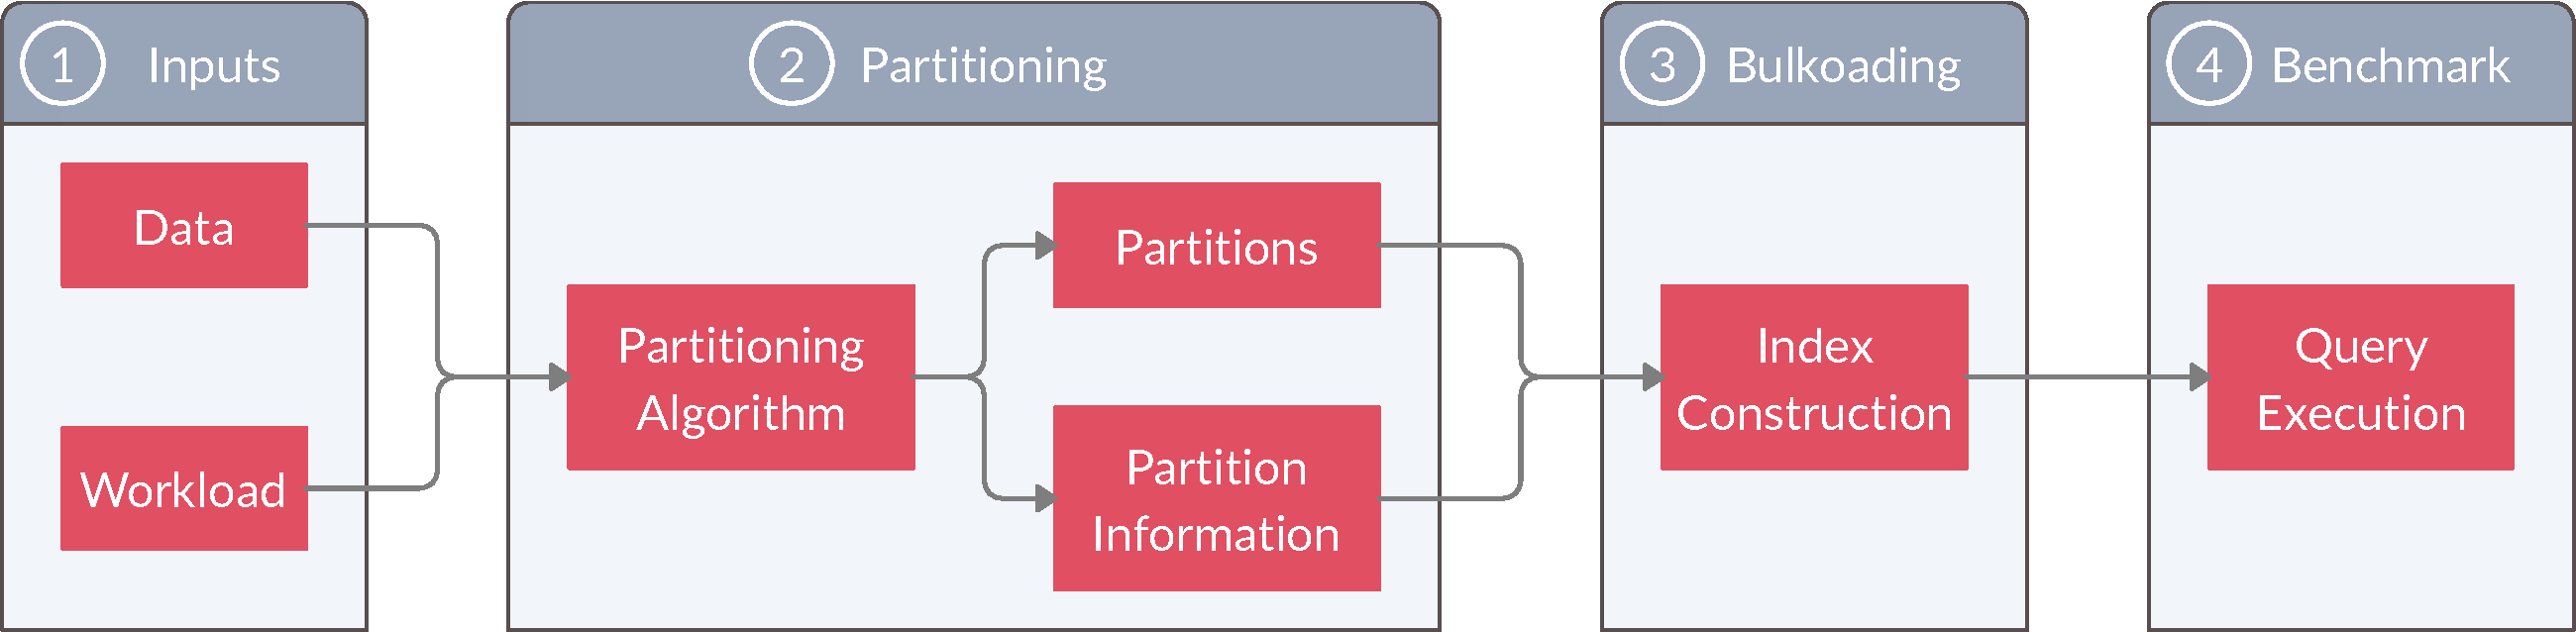
\includegraphics[width=\textwidth]{figures/pipeline.pdf}
    \caption{Framework Overview}
    \label{fig:framework}
\end{figure}

\section{Overview}
As we can see in \Cref{fig:framework}, the origin of all processes is the underlying data that we want to index and a query workload. However, we can also generate our own workloads through a Python script inside a Jupyter notebook. There, we can specify properties like the distribution and type of queries (point, range) that should be generated to access the data through the index. Because we wanted a fast workflow of generating and visualizing, we chose this approach. It has, however, the disadvantage that the workloads have to be saved to a file such that later on, the benchmarks can access them. Before they are saved, however, the queries generated in this step are divided into a train and test workload. The test workload will later be used in the C++ benchmarking.

Given the train workload, the partitioning algorithms that are described in \Cref{sec:frequency} and \Cref{sec:purity} can analyze the corresponding properties of the workload and will produce a partitioning of the underlying data. The resulting partitions are then saved to a file with additional information about each partition that can be used for the index construction. This information contains the relative frequency of a segment compared to the others and whether the segment mostly received point queries.
With these partitions, the index is bulkloaded from the data where each partition corresponds to an individual leaf node. The additional information is used to modify our index's structure and physical specialization. For example, if only point queries access a segment, it could be beneficial to manage data access through a hash table instead of a normal B-tree leaf. The next step is to execute the test workload on the index and compare it to other state-of-the-art indexes that were introduced in \Cref{sec:related_work}, namely a B$^+$-tree, an Adaptive Radix Tree (ART), and a Piecewise Geometric Model index (PGM).

\section{Workload Generation} \label{sec:wklgeneration}
The ultimate goal of this work is to generate a good partitioning for the index construction like it was mentioned in \Cref{bg:hybrid}. The inputs to the partitioning algorithms are, therefore, a dataset and a workload sample which we know is representative of the expected workload. However, to evaluate and test the algorithms and modifications, we required a flexible way to generate workload data, especially since it proved hard to find available real-world workload data. Although we do not have real-world workload data, we used our synthetic workload generation on real-world datasets in the hope that we get representative results. The workload generation is done in a Python script specifying a series of \verb|Region| objects. We have a basic repertoire of distributions (like uniform, zipfian, ...) that we append or overlap to create many different and more complex workloads. The \verb|Region| objects contain the following information:

\begin{itemize}
    \item \verb|index|: Whether the generation happens index-based or domain-based. Index-based means that we draw valid indices according to a distribution and then resolve the data values at these indices, domain-based means that we draw from the data domain, i.e.~we can draw values that fall inside the domain but are not present in the data itself. This cannot happen for an index-based generation.
    \item \verb|min, max|: The minimal and maximal values that indicate the region boundaries. In the index-based setting, these represent two indices that form the boundaries of this region. If we are in the domain-based setting, they represent the range of values from the data domain from which values can be generated.
    \item \verb|qtype|: The query type that should be generated in this region, e.g.~point or range queries
    \item \verb|num|: The number of queries in this region
    \item \verb|distribution|: The distribution underlying the generated queries in the region, e.g.~normal, uniform, ...
\end{itemize}

This gives us a very flexible way to generate arbitrary workloads. Note that while the partitions returned by our partitioning algorithms are mutually disjoint, the \verb|Region| objects used for workload generation do not need to be disjoint. This only means that we can overlap the boundaries of the objects to generate even more flexible workloads. In fact, it is the only way to generate regions of the data that are accessed through multiple types of queries, e.g.~through both point and range queries. 

As an example, \Cref{lst:generation} shows the code that would be used to generate a bimodal distribution of point queries. This is achieved by overlapping the two specified regions so that the two normal distributions form a bimodal distribution. The overlap is achieved by specifying the \verb|min| and \verb|max| attributes such that the \verb|max| of the first distribution is greater than the \verb|min| of the second distribution. In this case, the first normal distribution covers the first 70\% of the keys and the second distribution covers the last 70\% of the keys. 40\% of the keys in the middle will receive queries generated from both the first and the second distribution. The corresponding query distribution can be seen in \Cref{fig:bimodal}. Of course, the query distribution  depends on the data distribution it is applied to. While the data distribution in the first row was uniform to show the shape of the query distribution, the second row shows the same query distribution when sampling from exponentially distributed data.

\begin{lstlisting}[language=Python, caption=Example workload generation from Region objects, label=lst:generation]
    regions = [
        Region(
            qtype=QueryType.POINT, 
            num=100000, 
            distribution=DistributionType.NORMAL, 
            index=True, 
            min, max = 0, 0.7*len(data)
        ),
        Region(
            qtype=QueryType.POINT, 
            num=100000, 
            distribution=DistributionType.NORMAL, 
            index=True, 
            min, max =0.7*len(data), len(data)
        )
    ]
    wkl = Workload.from_regions(data, regions)
\end{lstlisting}

\begin{figure}
    \centering
    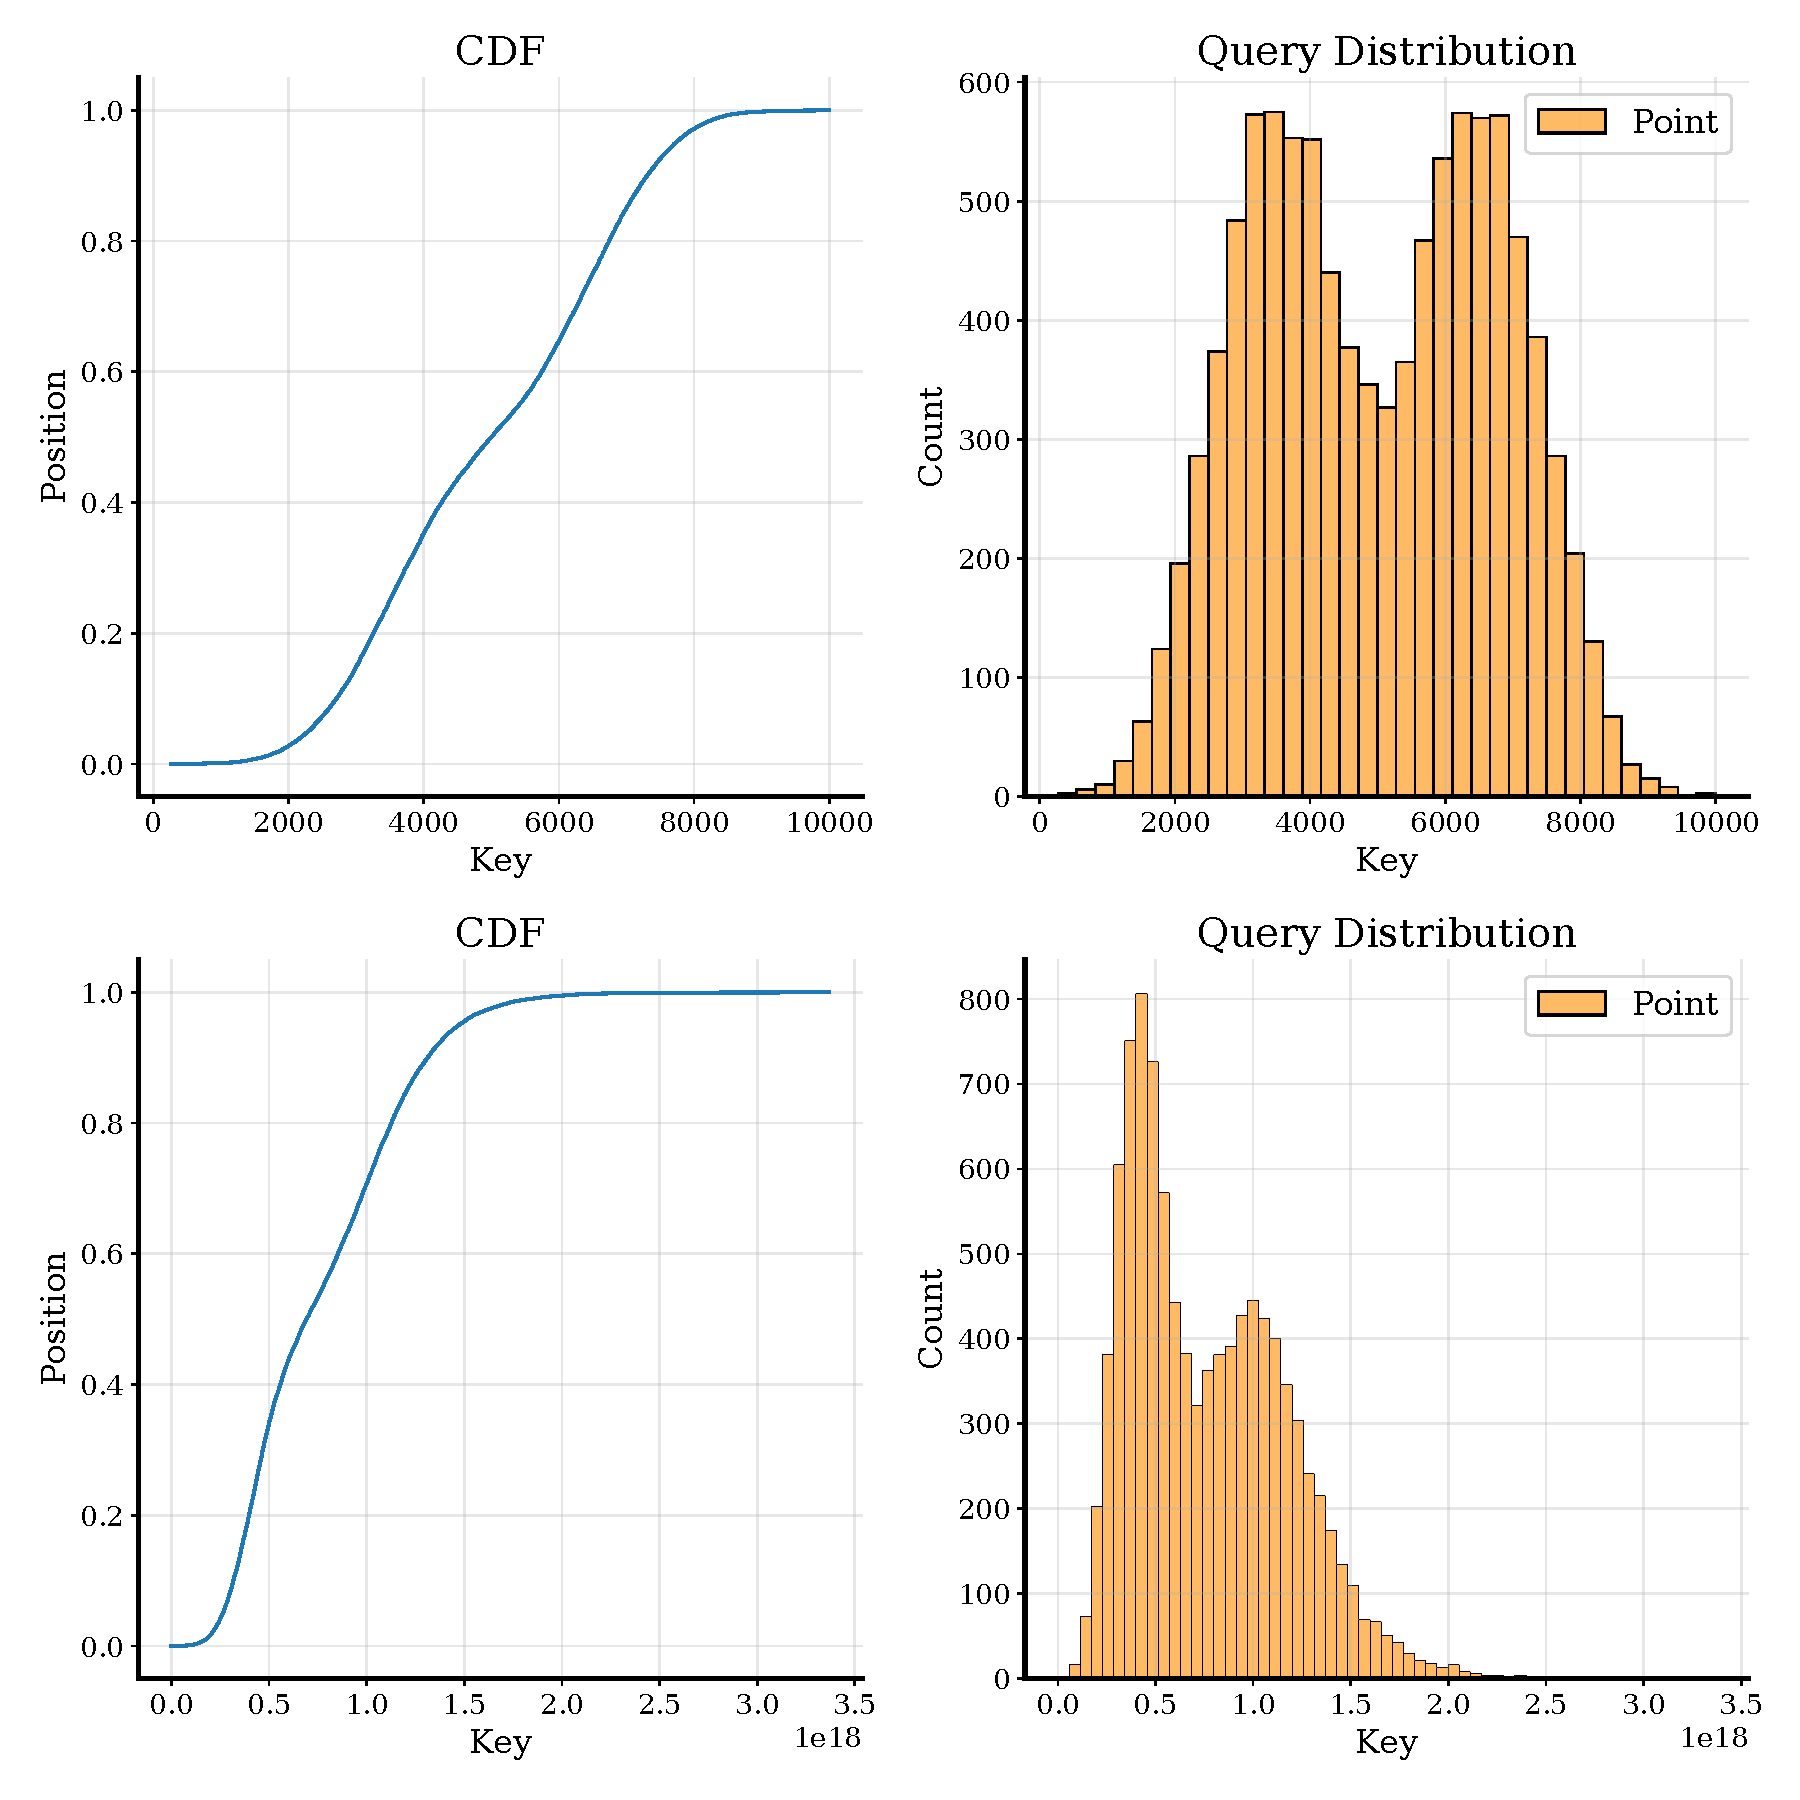
\includegraphics[width=\textwidth]{figures/bimodal.pdf}
    \caption[uniform and exponential query distributions after bimodal sampling]{CDF and query distribution of a bimodal workload on uniformly (top) and exponentially (bottom) distributed data}
    \label{fig:bimodal}
\end{figure}

After the queries are generated, we randomly sample a given fraction of them and remove these from the original queries. Similar to Machine Learning methods, we only use one of the resulting two sets to create our partitioning (training); the second set is later used for evaluation (testing) and immediately saved to a file. This ensures that we do not just design optimal partitions for the training queries. Instead, the partitions should be suitable for the underlying population of which train and test workload are only samples.

\section{Partitioning algorithms}
The next step in the framework is to use the train workload to find partitions in the data. There are many properties that one could look at when analyzing query workloads, but inspired by the works in \Cref{sec:related_work}, we decided to focus on two properties and look at how we could use these to partition the data and create segments: Frequency and Purity.

\subsection{Partitioning by Frequency} \label{sec:frequency}
The first algorithm analyzes the frequency of query accesses for each key in our dataset. The motivation behind using the frequency as a partition property is that, hopefully, we can benefit from caching effects during the execution of the test workload. We hope that the path to highly frequent segments remains in the cache so that subsequent queries can retrieve the location of the corresponding keys faster. On the other hand, the path to rarely touched segments should not be present in the cache most of the time. Additionally, by analyzing the frequency, we can use that information to change the structure of the index. The first idea in this regard would be to shift highly frequent segments higher up in the tree, to prevent expensive pointer chasing when traversing the index.

We first realized that traversing our data key-by-key and comparing them with each other is not useful for a generalizing partitioning algorithm because we can only operate on a train workload that is sampled from the general workload distribution. If we used these key-by-key comparisons for the frequency to create partitions, we would probably overfit the patterns in the train workload, even though these might only be caused by noise and not be present in the general distribution. Therefore, we employ an approach that tries to maximize the previously mentioned goal: find partitions where keys are accessed roughly the same amount of times. Regions with almost no query accesses will be put in one partition, resulting in the segment not being loaded very often. On the other hand, regions with similarly frequent keys will result in the  corresponding segment remaining in the cache if the frequency is high enough. However, one downside to this approach is that segments could become very large. As all information about a partition is contained in a single leaf node, large segments will prevent them from being cached entirely, as they are simply too large to fit in the cache. Still, parts of the node may remain in the cache. Additionally, we can hope that the inner nodes on the path between the root node and this leaf node remain completely in the cache since their size is fixed.

As already described in \Cref{bg:numerical}, we want to use finite difference approximations to estimate the derivative of the frequency our keys are accessed. Since the key space is discrete, the frequency function is discrete, so using the finite difference approximations is appropriate. We designed a single-pass algorithm that tries to find plateaus in the workload distribution by calculating the average change in frequency over a sliding window. It uses three phases depending on where it currently is concerning a plateau, which is heavily inspired by the three different approximations. As we have mentioned before, we do not want to use key-by-key comparison, as this is very sensitive to outliers. However, our finite difference approximations would do this: For example, the forward approximation would compare the current frequency to the frequency of the key with distance $h$ away. Instead of doing this, we compare the current frequency to the average frequency of the keys from the current key up to $h$ keys further away. Averaging over all these keys will enable us to generalize better and avoid starting new segments at outliers. The three phases are therefore:

\begin{enumerate}
    \item[I.] Start calculating a discrete forward difference approximation. As only keys "in the future" are considered, this phase is predestined to find an incoming plateau by checking if the calculated slope is near zero.
    \item[II.] After such a plateau was found, we used the central difference approximation to establish the boundaries of the plateau. We use this approximation now, as it considers keys from before and after the current one. This should give a better estimation of when a plateau is ending.
    \item[III.] Once the central approximation indicates that a plateau is ending (with an approximation value further away from zero), we switch to calculating the backward finite difference approximation to ensure that we find the exact end point of the plateau. We only consider previous keys, as we now know that an end is coming, giving us the best chance to catch the key responsible for significantly changing the slope.
\end{enumerate}


\begin{algorithm}
\caption{Partition by Frequency}\label{algo:freq}
\begin{algorithmic}[1] 
    \Procedure{PartitionFrequency}{$data, w, \delta$}
    \State $idx \gets 0,$ \; $n \gets data.size$ \; $w' \gets \lfloor \frac{w}{2} \rfloor$
    \While{$idx < n - w$} \Comment{Start Phase I}
        \State $falseAlarm \gets \text{False}$
        \State $fwdSlope \gets$ \textsc{ForwardDiff}($data, idx, idx + w$)
        \If{$| fwdSlope | \leq \frac{\delta}{w}$} \Comment{Potential partition start}
            \State $potStart \gets idx$
            \State $idx \gets idx + 1$
            \For{$i \gets 1$ to  $ w'$} \Comment{Start Phase II}
                \State $centralSlope \gets$ \textsc{CentralDiff}($data, idx - i, idx + w'$)
                \If{$| centralSlope | > \frac{\delta}{w}$}
                    \State $falseAlarm \gets$ True \Comment{Enforce minimal partition size}
                \EndIf
                \State $idx \gets idx + 1$
            \EndFor
            \If{\textbf{not} $falseAlarm$} \Comment{Plateau large enough}
            \State \textsc{Append}($result, potStart$)
            \While{$idx < n - \lfloor \frac{w}{2} \rfloor$} \Comment{Continue Phase II}
                \State $centralSlope \gets$ \textsc{CentralDiff}($data, idx - w', idx + w'$)
                \If{$| centralSlope | > \frac{\delta}{w}$}
                    \State\textbf{break} \Comment{Near end of plateau, go to Phase III}
                \EndIf
                \State $idx \gets idx + 1$
            \EndWhile
            \While{$idx < n - w$} \Comment{Start Phase III}
                \State $bwdSlope \gets$ \textsc{BackwardDiff}($data, idx - w, idx$)
                \If{$| bwdSlope | > \frac{\delta}{w}$}
                    \State \textsc{Append}($result, idx$) \Comment{End of plateau found}
                    \State\textbf{break} \Comment{Back to Phase I}
                \EndIf
                \State $idx \gets idx + 1$
            \EndWhile
            \Else \Comment{Plateau was not large enough}
            \State $idx \gets potStart + 1$ \Comment{Start over at Phase I}
            \EndIf
        \Else
            \State $idx \gets idx + 1$ \Comment{No small forward approx., go to next key}
        \EndIf
    \EndWhile
    \State \textsc{Append}($result, n$) \Comment{Add last boundary to $result$}
    \State \textbf{return} $result$
    \EndProcedure
\end{algorithmic}
\end{algorithm}

These phases can be mapped to \Cref{algo:freq}. The input to this algorithm is the data we want to partition, a window size parameter $w$ for the sliding window, and $\delta$ to control the strictness of what is still considered a plateau. After initializing our variables at the start (line 2), we begin to go over our keys as long as we can compute a forward difference approximation (line 3). We compute the forward difference approximation as described above, and if we may have found a plateau, we start the second phase (lines 6-8). However, to ensure that not every time we encounter a zero forward difference approximation, we start a new partition, we require that for the next $\lfloor \frac{w}{2} \rfloor$ keys, the central approximation stays close to zero (lines 6-15). This value was chosen purely heuristically. The variable $falseAlarm$ keeps track of whether our potential plateau is large enough. If it is not, we go back to phase one, beginning one key after the previous potential start (lines 33-35). This approach will cause the partitions to be at least $\lfloor \frac{w}{2} \rfloor$ keys long. If all the central approximations were near zero, we append this partition to our result (line 17). Then, we continue to calculate the central difference approximation as long as we see near zero values. Should this no longer be the case, we change to phase three with the backward difference approximation (lines 18-24). As soon as this backward difference approximation also becomes deviates too much from zero, we determine that the plateau has ended and therefore start a new partition (lines 25-32). If we initially did not have a small enough forward approximation for our current index, we just start over with the next key (lines 36-38). In the end, we append the last index to our partitions, as our convention is that the index representing the partition is the last index of the partition (line 40).

\subsection{Partitioning by Purity} \label{sec:purity}
The second algorithm does not analyze the frequency of a key but the query types that access the key. This way, we can distinguish between keys that are not requested at all by queries, those that are only accessed by one single type (e.g.~point or range queries), and those that are accessed by different types (e.g.~accessed through point and range queries, each). The motivation behind this approach is that we can use this information to adapt our hybrid index structure such that the underlying data structure is optimized for certain sub-ranges. One optimization that comes to mind is using a hash table for a segment that is only accessed through point queries. One can benefit from the faster lookup time, while the disadvantage of hash tables, the unsortedness of the keys, has no impact because we know that we have no range queries that access this segment.

Like the frequency algorithm above, we ruled out the use of key-by-key comparisons because of the generalization problem. Instead, we used a rather simple algorithm that tries to find the boundaries where the query type changes. The goal here is to determine partitions with pure access patterns, so one partition should mostly contain one query type (or only mixed accesses). The algorithm is a single-pass over the data, where we again consider a sliding window around the currently selected key. For each key, we store the predominant query type in that window, and as soon as we have a different major query type than for the previous key, we begin a new partition. We opted to use this simpler approach here, as we look at the mode of the query types in a certain window. While outliers in the frequency domain have the potential to change the average frequency significantly, an outlier in the query type will not affect the mode. However, we note that while a single range query in a region with otherwise only point queries does not affect the mode, it could still incur a significant performance cost later on because a range query is more expensive to perform on e.g.~hash tables.

In \Cref{algo:purity} we initialize our index at the point $\lfloor \frac{w}{2} \rfloor$, as we want to be able to calculate the mode across one whole window, which automatically means that the first $\lfloor \frac{w}{2} \rfloor$ keys always belong to the same partition (lines 2-3). We then calculate the mode across the query types for this window and proceed with the next key (lines 5-6). While we can still create a full window, we calculate the mode for this window, and if it differs from the previous key's mode, we end our partition (lines 7-11). Lastly, we need to update the variable that holds the previous key's mode to the current one and proceed with the next key (lines 12-13). In the end, we append the last index to conclude the last partition, as per our convention mentioned before (line 15).

\begin{algorithm}
\caption{Partition by Purity}\label{algo:purity}
\begin{algorithmic}[1]
    \Procedure{PartitionPurity}{$data, w$}
    \State $w' \gets \lfloor \frac{w}{2} \rfloor$
    \State $idx \gets w'$
    \State $n \gets data.size$
    \State $lastMode \gets$ \textsc{CalculateMode}($data, idx - w', idx + w'$)
    \State $idx \gets idx + 1$
    \While{$idx < n - w'$}
        \State $curMode \gets$ \textsc{CalculateMode}($data, idx - w', idx + w'$)
        \If{$curMode \neq lastMode$}
            \State \textsc{Append}($result, idx$)
        \EndIf
        \State $lastMode \gets curMode$
        \State $idx \gets idx + 1$
    \EndWhile
    \State \textsc{Append}($result, n$)
    \State \textbf{return} $result$
    \EndProcedure
\end{algorithmic}
\end{algorithm}

\section{Index Bulkloading and Benchmarking}
To understand how we incorporate the partitioning information into our index, we need to cover the general structure of the hybrid index and how it is built and bulkloaded before being benchmarked. Additionally, we look at how the index is altered by the partition information.

\subsection{Structure of the index}
The general structure of our index is very similar to the indexing framework presented by \citeauthor{Dittrich2021} \cite{Dittrich2021}. Our index has the same internal structure as a B$^+$-tree, but we do not fix the size of the leaf nodes. Instead, each leaf is designed to represent exactly a partition produced by the partitioning algorithms from before. As described in \Cref{bg:hybrid}, we have the flexibility to choose the data layout and search strategy inside each node separately. The default search strategy for the internal nodes (to locate the next child) and the leaf nodes (to locate the final position) was chosen as binary search, as we deal only with sorted data in this work. This restriction was applied here because if we were to partition unsorted data and obtain some partitions, their ranges (minimum and maximal value inside partition) would certainly not be disjoint. However, this characterizes the routing inside a B$^+$-tree-like structure. As this requirement would not be satisfied, we could not use the described internal tree-like structure, and it is not immediately clear how the routing inside the index needs to be designed to support such partitions. Therefore, we did not look into the case of partitioning unsorted data.

\subsection{Choice of leaf data structure}
The first way of optimizing our index given the partition information is to change the leaf data structure that is used to map the keys of our dataset to their positions. The default choice of a binary search with a sorted layout is well suited for a general workload where we would anticipate range queries, as we only need a lower bound point query and an additional scan towards the upper bound to determine all keys that qualify for the query. This is a sensible default, but we choose to use a hash table instead for a point query-only segment. As mentioned before, we achieve a better lookup performance for point queries, and as there are (almost) no range queries in the segment, we do not need to support an efficient lookup for them. Should we encounter a range query in the test workload, we can still guarantee the correctness of the results by converting the range query to a series of point queries that can be executed on the hash table. While this optimization seems straightforward, we could also change the leaf data structure for other different scenarios, although that was not further explored in this work.

\subsection{Transforming leaf nodes} \label{sec:leaftransform}
The next way of optimizing the index is to utilize the frequency of the partitions that are generated more effectively. Apart from only creating the partitions, one could also consider improving access times for frequently visited segments. One way of doing so was presented in \Cref{sec:related_work}, where the authors adaptively classified nodes as hot or cold based on current and past access statistics. Then they either applied a performance-optimized or space-optimized encoding to these nodes, depending on the classification. In the framework presented in \Cref{bg:hybrid}, this would correspond to a node mutation, where compression would be chosen and applied. Another approach that we wanted to look into is moving the leaf segments with a relatively large frequency higher up in the tree, which would result in a shallower path to the corresponding segment in our index. We suspect that we could benefit from caching effects here, as there are fewer nodes above the leaf segment that need to remain in the cache for faster access. This approach can be seen in \Cref{fig:frequencybulkload}. The top half shows the resulting index after bulkloading the data points 1, 4, 7, ..., 27, 29, and 30. A standard bulkloading approach starts by constructing the leaf nodes and proceeds with constructing inner nodes in a bottom-up fashion. In our example, the bulkloading would collect the three left-most leaf nodes to construct the left inner node one level higher up. The remaining leaf nodes would then be put in a second inner node because the first one ran out of capacity. However, if we knew that the keys in the third leaf node are frequently requested, we could decide to push this leaf node to a higher index level as done in the bottom half. In our example, we treat our leaf node as if it was an inner node one level higher up. We then need to construct the other inner nodes for this level, but we cannot treat the remaining leaf nodes as if they were only one instance of the bulkloading. If we did this, the left inner node would fill up to capacity and include the leaf node with keys 19, 22, and 24. This would result in two inner nodes whose ranges are no longer disjoint because the left one would include keys from 1 to 24, while the middle one (our original leaf) has a range from 14 to 18. Therefore, we treat the leaf nodes left from our original one and right from it as separate sub-problems to the bulkloading. The resulting inner nodes can then be treated as siblings to our original leaf node, which ensures that ranges of nodes on the same level are disjoint. At this point, we need to note that while we describe this approach here, we did not have enough remaining time to implement it and use it in our experiments.

\begin{figure}
    \centering
    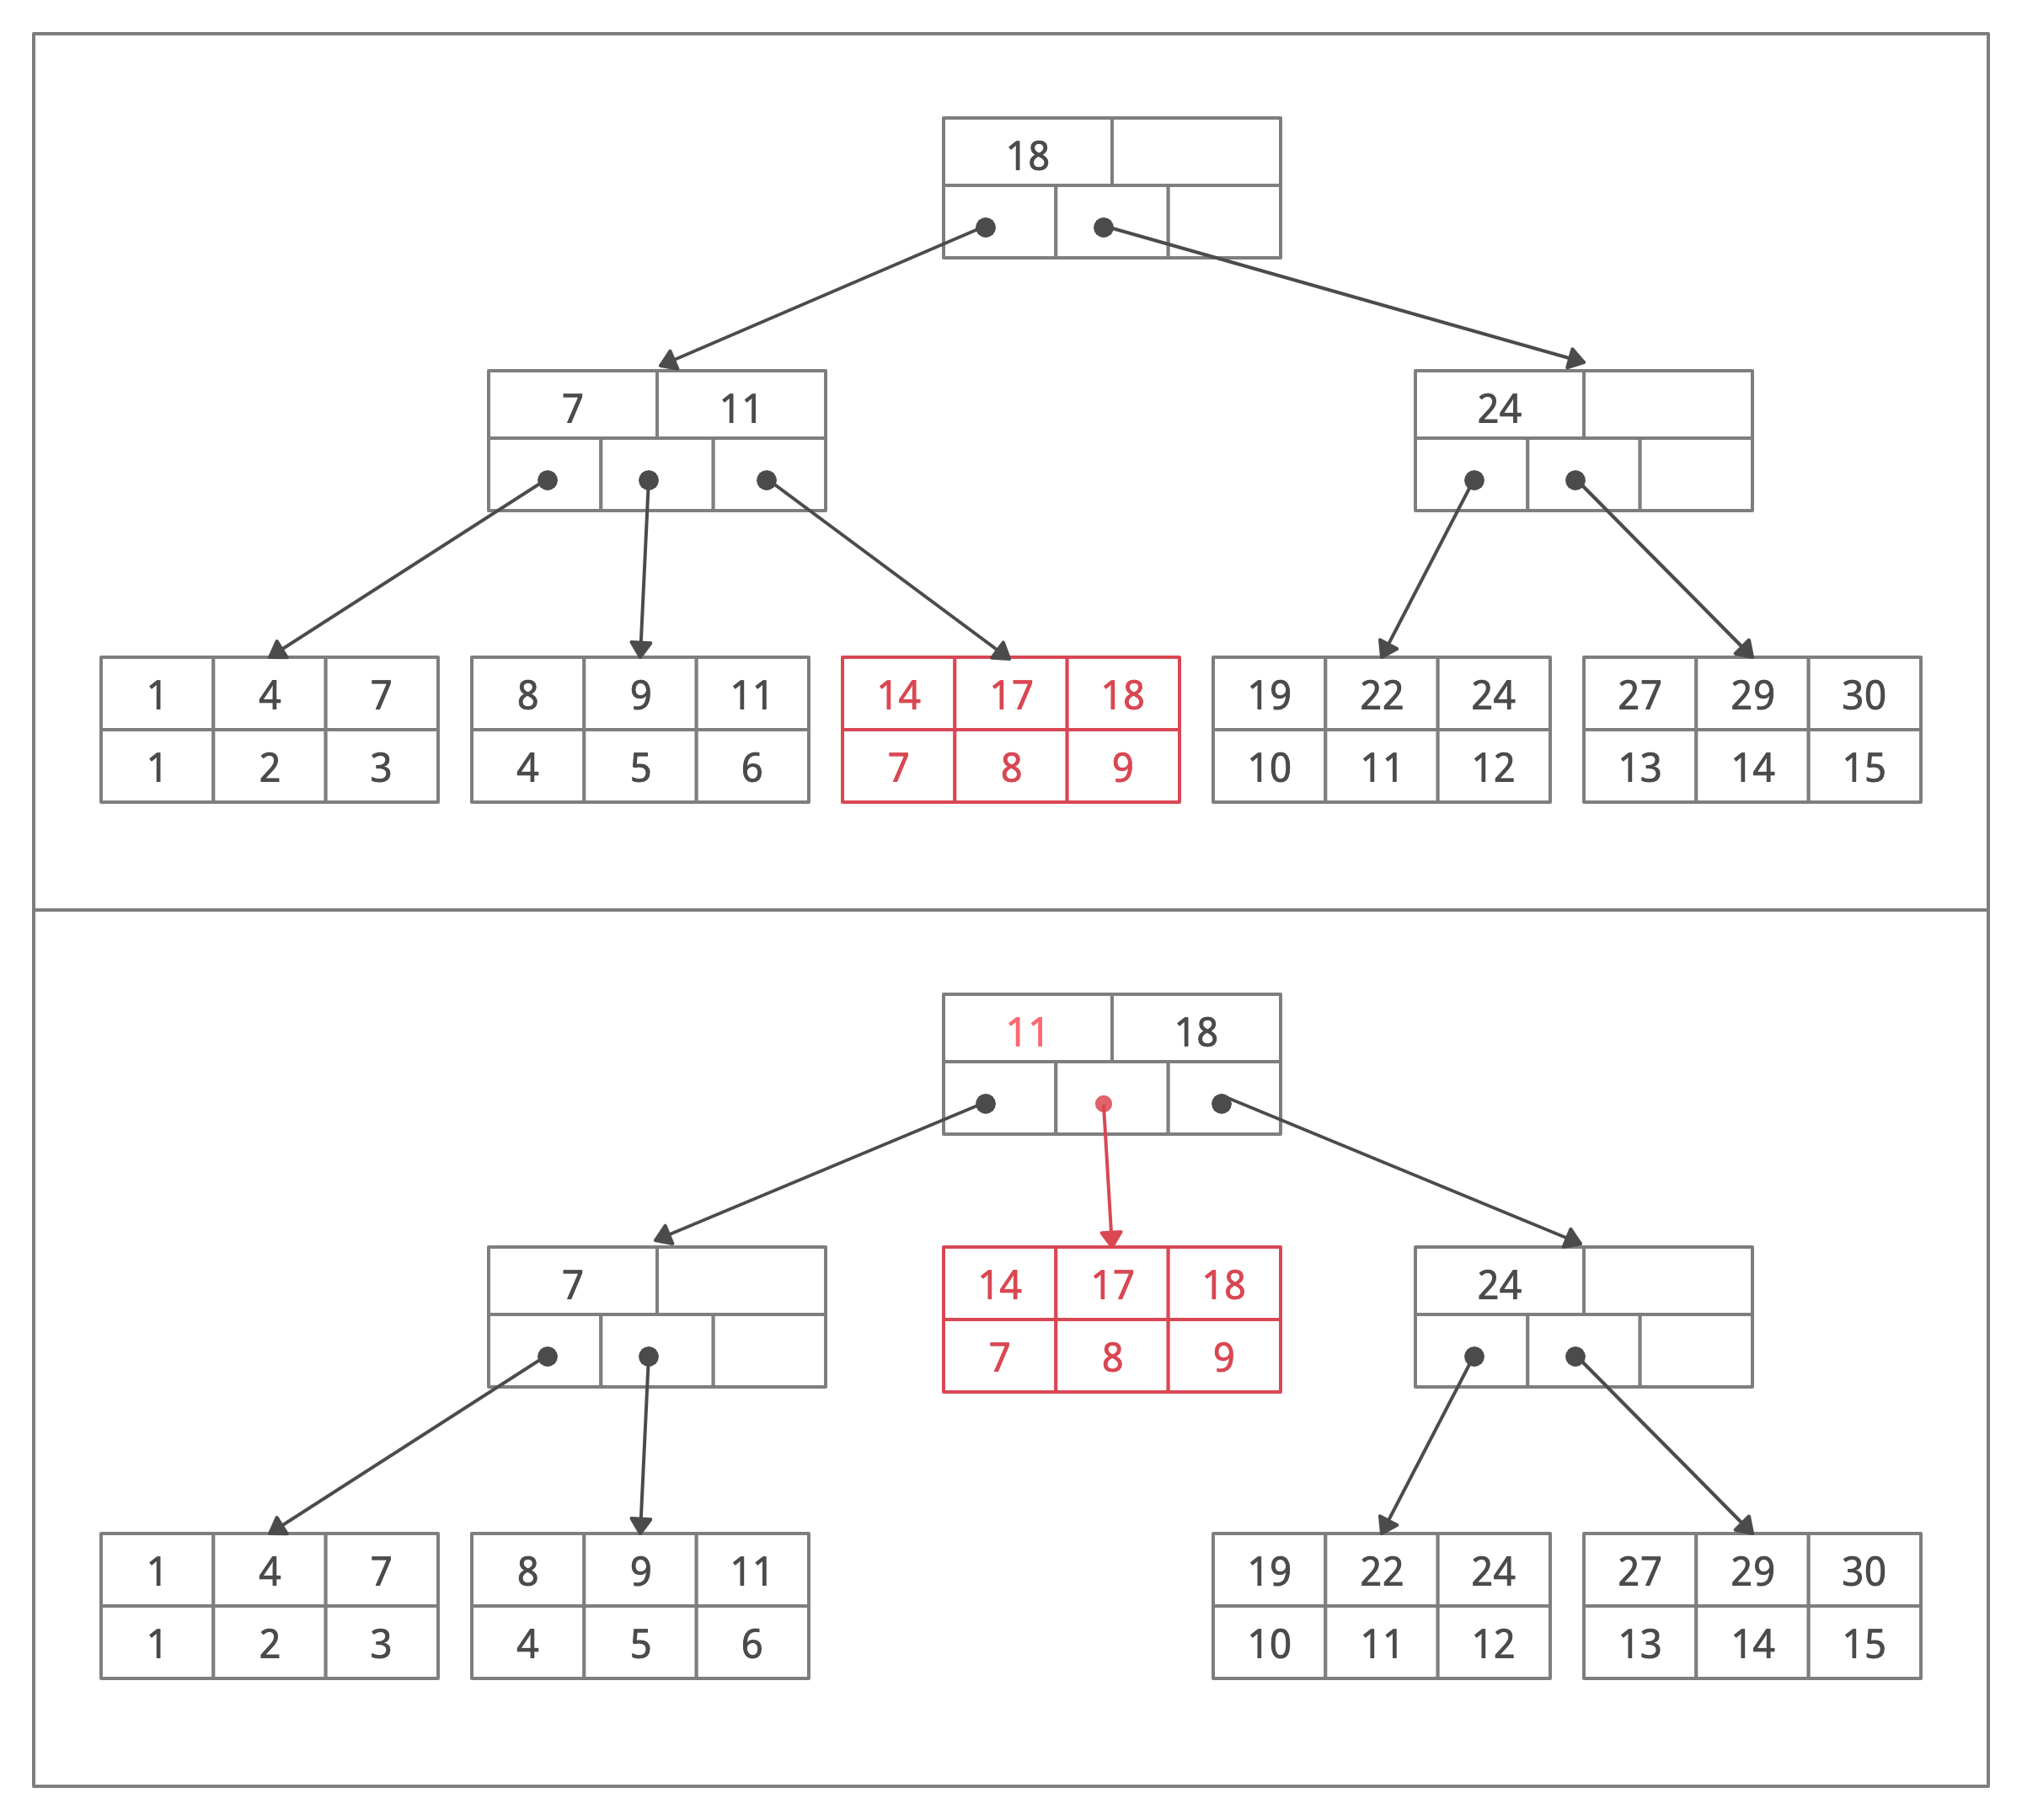
\includegraphics[width=\textwidth]{figures/frequency_bulkloading.png}
    \caption[Incorporating frequency information into index bulkloading]{Resulting index after standard bulkloading (top) and after bulkloading with additional frequency information (bottom)}
    \label{fig:frequencybulkload}
\end{figure}